%==============================================================================
% Sjabloon poster bachproef
%==============================================================================
% Gebaseerd op document class `a0poster' door Gerlinde Kettl en Matthias Weiser
% Aangepast voor gebruik aan HOGENT door Jens Buysse en Bert Van Vreckem

\documentclass[a0,portrait]{hogent-poster}

% Info over de opleiding
\course{Bachelorproef}
\studyprogramme{toegepaste informatica}
\academicyear{2024-2025}
\institution{Hogeschool Gent, Valentin Vaerwyckweg 1, 9000 Gent}

% Info over de bachelorproef
\title{Hoe beïnvloeden data-partitioneringstechnieken in combinatie met edge-databases de prestaties van een Edge Computing-omgeving bij Optis?}
% \subtitle{Ondertitel (eventueel)}
\author{Wout Van Cleemput}
\email{wout.vancleemput@student.hogent.be}
\supervisor{Karine Samyn}
\cosupervisor{Kenneth Van den Berghe (Optis)}

% Indien ingevuld, wordt deze informatie toegevoegd aan het einde van de
% abstract. Zet in commentaar als je dit niet wilt.
\specialisation{Systeem- en Netwerkbeheer}
\keywords{Edge Database, Edge Computing, Data Partitioning}
\projectrepo{https://github.com/WoutVC/bachelorproef2024}

\begin{document}

\maketitle

\begin{abstract}
  Deze bachelorproef richt zich op de invloed van data-partitioneringstechnieken en edge-databases op de prestaties van een Edge Computing-omgeving, met een specifieke focus op de toepassing bij Optis.

  Het doel is om praktische aanbevelingen te formuleren voor Optis door de impact van verschillende partitioneringstechnieken op databaseprestaties te analyseren binnen een simulatie. 
  
  Dit onderzoek helpt bij het begrijpen van de toepasbaarheid van partitionering in schaalbare omgevingen en levert praktische inzichten die door Optis kunnen worden toegepast.
  
  Om een grondige basis te leggen, werd een uitgebreide literatuurstudie uitgevoerd naar bestaande Edge Database-technologieën en data-partitioneringstechnieken.
  
  Op basis van deze inzichten werd er een Proof of Concept aangemaakt. In deze PoC gebruikten we een testomgeving waarin verschillende databases zoals Cassandra, MongoDB en TimescaleDB werden geëvalueerd op belangrijke prestaties zoals latentie, throughput, schaalbaarheid en fouttolerantie.
  
  Het onderzoek biedt een combinatie van theoretische en praktische bijdragen, waaronder een duidelijk overzicht van de huidige ontwikkelingen binnen Edge Database-architecturen met bijzondere aandacht voor de vereisten van organisaties zoals Optis.
  
  De resultaten dragen bij aan de verbetering en toepassing van Edge Computing-technologieën in verschillende sectoren.
\end{abstract}

\begin{multicols}{2} % This is how many columns your poster will be broken into, a portrait poster is generally split into 2 columns

\section{Introductie}



\section{Experimenten}

\section{Resultaten}

\begin{center}
  \captionsetup{type=figure}
  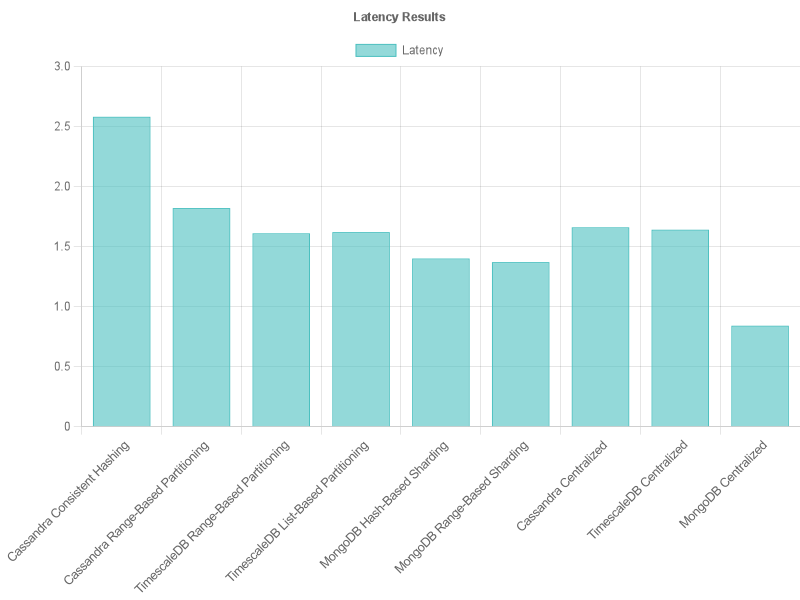
\includegraphics[width=0.75\linewidth]{Latency.png}
  \captionof{figure}{Vergelijking van latentie tussen Cassandra, MongoDB en TimescaleDB.}
\end{center}

\paragraph{Analyse van latentie:}
De grafiek laat zien dat \textit{MongoDB (Range-Based Sharding)} met een latentie van 1.37 ms de laagste latentie behaalt, wat het geschikt maakt voor toepassingen met hoge snelheidseisen. \textit{Cassandra (Alternative Range-Based Partitioning)} scoort eveneens goed met 1.82 ms. \textit{TimescaleDB (Range-Based Partitioning)} presteert met een latentie van 1.61 ms relatief goed, maar is minder efficiënt dan MongoDB.

\begin{center}
  \captionsetup{type=figure}
  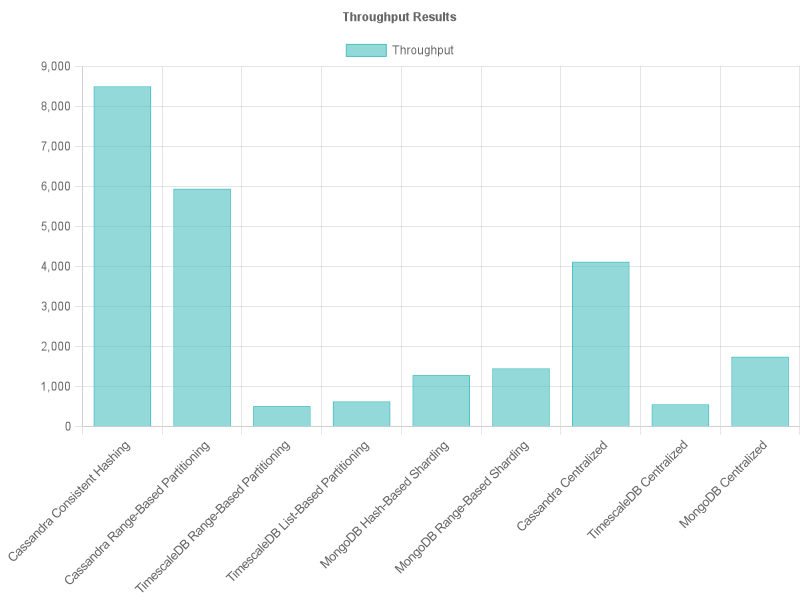
\includegraphics[width=0.75\linewidth]{Throughput.png}
  \captionof{figure}{Vergelijking van throughput tussen Cassandra, MongoDB en TimescaleDB.}
\end{center}

\paragraph{Analyse van throughput:}
\textit{Cassandra (Consistent Hashing)} behaalt de hoogste throughput met 8500.37 records per seconde, wat het ideaal maakt voor omgevingen met zware invoerbelastingen. \textit{MongoDB (Range-Based Sharding)} presteert redelijk met 1452.75 records per seconde. \textit{TimescaleDB (Alternative List-Based Partitioning)} heeft een significant lagere throughput van 628.02 records per seconde.

\begin{center}
  \captionsetup{type=figure}
  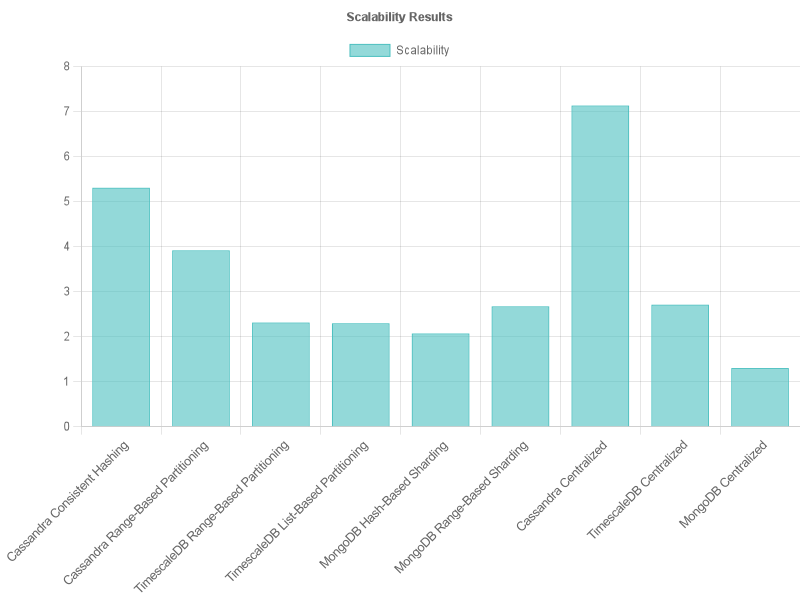
\includegraphics[width=0.75\linewidth]{Scalability.png}
  \captionof{figure}{Vergelijking van schaalbaarheid tussen Cassandra, MongoDB en TimescaleDB.}
\end{center}

\paragraph{Analyse van schaalbaarheid:}
Uit de grafiek blijkt dat \textit{Cassandra (Consistent Hashing)} de hoogste schaalbaarheid biedt met een score van 2.34, gevolgd door \textit{Alternative Cassandra (Range-Based Partitioning)} met 2.28. \textit{TimescaleDB (Range-Based Partitioning)} scoort lager met 1.53, wat wijst op beperkingen bij het schalen naar hogere workloads.

\begin{center}
  \captionsetup{type=figure}
  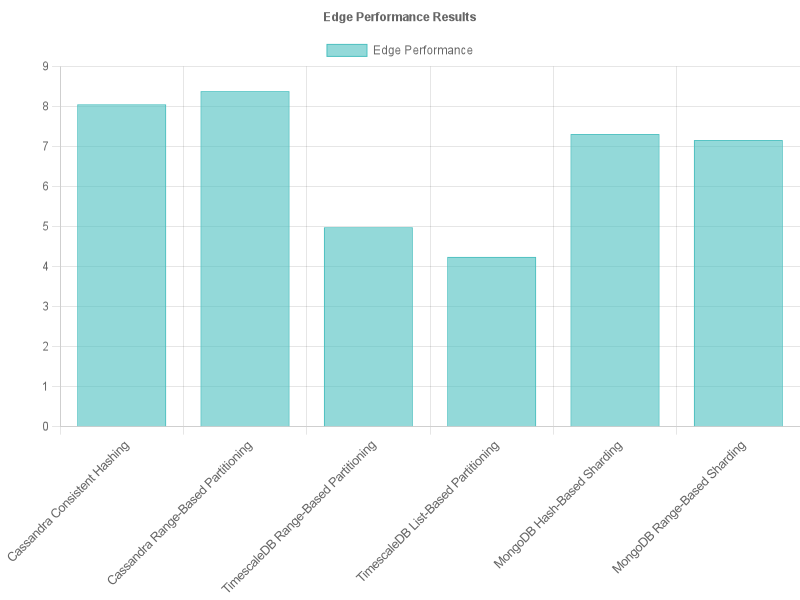
\includegraphics[width=0.75\linewidth]{Edge_Performance.png}
  \captionof{figure}{Vergelijking van edge performance tussen Cassandra, MongoDB en TimescaleDB.}
\end{center}

\paragraph{Analyse van edge performance:}
De grafiek toont aan dat \textit{Alternative Cassandra (Range-Based Partitioning)} de beste edge performance behaalt met 8.38, gevolgd door \textit{Cassandra (Consistent Hashing)} met 8.05. \textit{TimescaleDB (Alternative List-Based Partitioning)} scoort het laagst met 4.24.

\begin{center}
  \captionsetup{type=figure}
  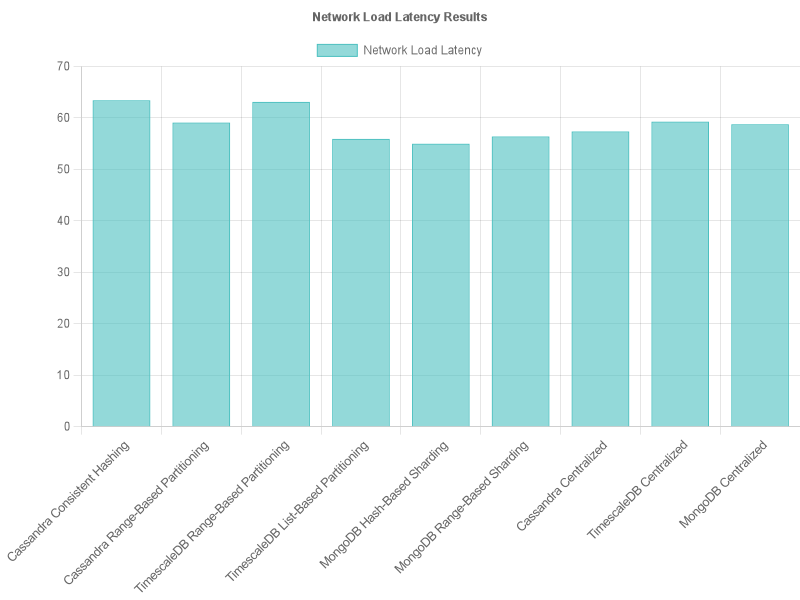
\includegraphics[width=0.75\linewidth]{Network_Load Latency.png}
  \captionof{figure}{Vergelijking van netwerklatentie tussen Cassandra, MongoDB en TimescaleDB.}
\end{center}

\paragraph{Analyse van netwerklatentie:}
Netwerklatentie wordt het laagst gehouden door \textit{MongoDB (Hash-Based Sharding)} met een score van 54.96, gevolgd door \textit{Alternative TimescaleDB (List-Based Partitioning)} met 55.91. \textit{Cassandra (Alternative Range-Based Partitioning)} toont een iets hogere score van 59.06, maar blijft stabiel onder hoge netwerkbelasting.

\section{Conclusies}

\begin{center}
	\captionsetup{type=figure}
	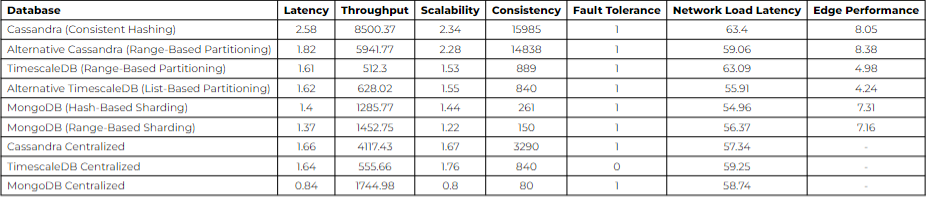
\includegraphics[width=1.0\linewidth]{Resultaten.png}
	\captionof{figure}{Samenvatting van de resultaten van de experimenten.}
  \end{center}

\section{Toekomstig onderzoek}

- Onderzoek naar hybride databasesystemen.
- Uitbreiding met meer fouttolerantie- en beveiligingstests.
- Integratie van edge computing met cloud-native applicaties.

\end{multicols}
\end{document}